\section{Linear Mixed-Effect Models}
\subsection{ Mixed-Effects Models}
\begin{frame}{Feature Selection for Mixed-Effect Models}

Mixed-effect models
\begin{itemize}
	\item Used for analyzing \textbf{combined data} across a range of \textbf{groups}.
	\item Use covariates to separate the \textbf{population variability} from the \textbf{group variability}.
	\item \textbf{Borrow strength} across groups to estimate key statistics. % when data within units are sparse or highly variable.
\end{itemize}

\begin{figure}
	\centering
	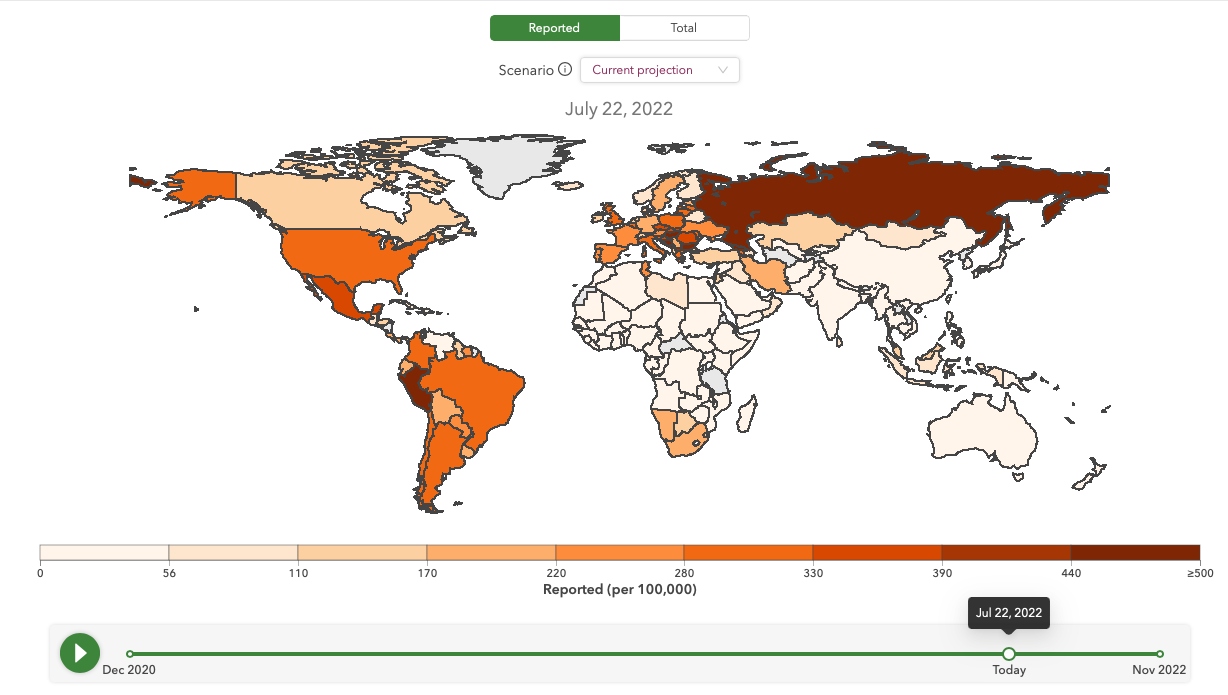
\includegraphics[width=0.8\textwidth]{Figures/ihme_predictions.png}\footnote{Picture is taken from \href{covid19.healthdata.org}{covid19.healthdata.org} }
\end{figure}

\end{frame}

\begin{frame}{Feature Selection for Mixed-Effect Models}
Practitioners:
\begin{itemize}
	\item Often seek \textbf{sparse models} that select \textbf{most informative} covariates. 
	\item Want to be \textbf{flexible but efficient} in using various sparsity-promoting terms.
	\item Want a library to be \textbf{universal and compatible} with e.g. \texttt{sklearn}.
\end{itemize}
\vspace{1em}

Sparse Relaxed Regularized Regression ($\mathcal{SR}3$) \cite{Zheng2018RelaxAndSplit} showed great results for t linear models:

\begin{figure}
	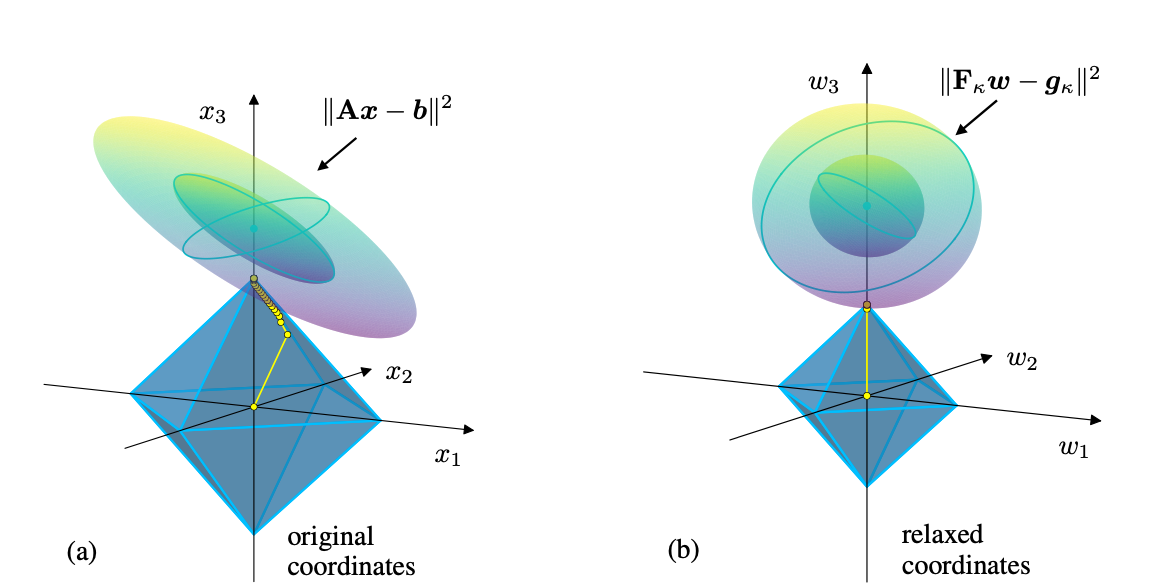
\includegraphics[width=0.7\textwidth]{Figures/intuition_prev_paper.png}
\end{figure}

\vspace{1em}
\textit{\textbf{Goal}: create a feature selection library that uses a relaxation approach for feature-selection in mixed-effect models.}

\end{frame}


\begin{frame}{Linear Mixed-Effect (LME) Models}

	Dataset: $m$ groups $(X_i, Z_i, y_i),\quad i = 1, \dots m$, each has $n_i$ observations
	\begin{itemize}
		\item 	$X_i \in \R^{n_i \times p}$ -- group $i$ design matrix for fixed features
		\item 	$Z_i \in \R^{n_i \times q}$ -- group $i$ design matrix for random features
		\item 	$y_i \in \R^{n_i}$ -- group $i$ observations  
	\end{itemize}
	

	\begin{columns}[T,onlytextwidth]
	
    \column{0.5\textwidth}
    \vspace{3em}
    Model:
	 	\[
   		\begin{split}
   			y_i & = X_i\beta + {\color{red}Z_i u_i} + \varepsilon_i \\
   			 \varepsilon_i & \sim \NN(0, \Lambda_i) \\
   			{\color{red} u_i} & {\color{red}\sim \NN(0, \Gamma)}
   		\end{split}
   		\]
   		
   	Equivalently:
   		\[
   		\begin{split}
   			y_i & = X_i\beta + \textcolor{red}{\omega_i} \\
   			{\color{red} \omega_i} & {\color{red}\sim \NN(0, Z_i\Gamma Z_i^T + \Lambda_i)}
   		\end{split}
   		\]
   	
   	Simplifying assumption: 
   	\[
   		\Gamma = \diag(\gamma)
   	\]
   	
    \column{0.5\textwidth}
    	\centering  
   	\begin{figure}
   		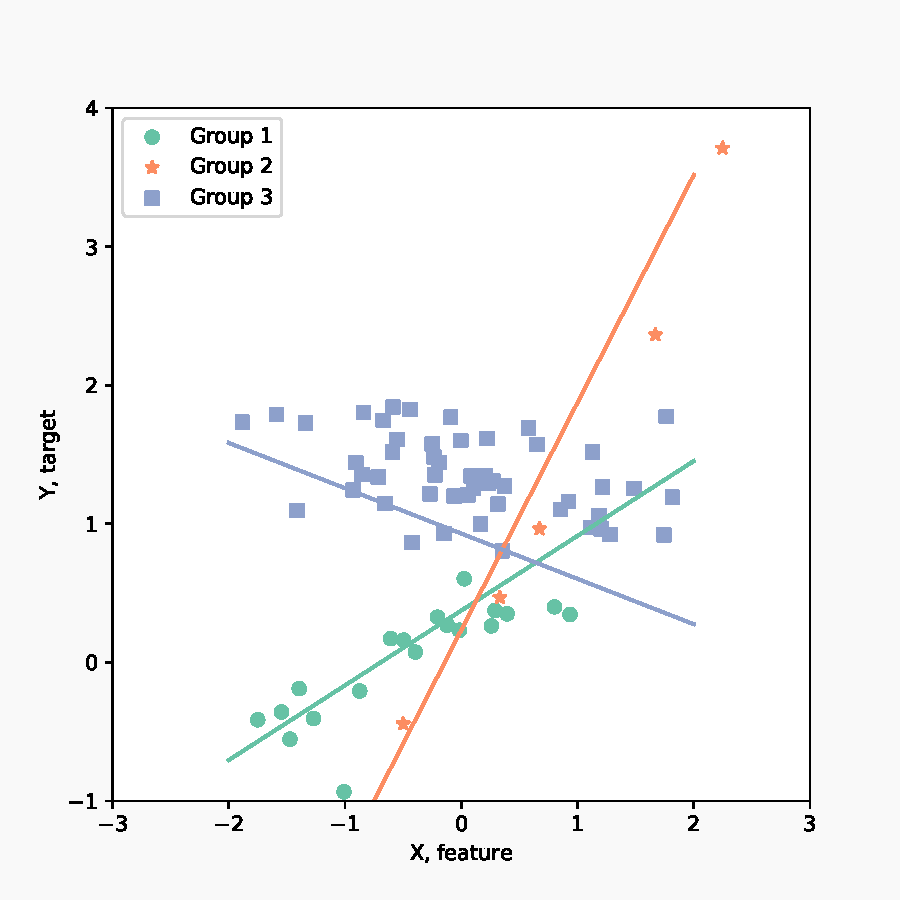
\includegraphics[width=0.9\textwidth]{Figures/lme_example_random_prediction}
   	\end{figure}
   	   		

   	
  \end{columns}
\end{frame}

\begin{frame}{Notation}
	\eq{
   		y_i & = X_i\beta + Z_iu_i + \varepsilon_i \quad i = 1\dots m \\
   		\varepsilon_i & \sim \NN(0, \Lambda_i) \\
   		u_i & \sim \NN(0, \Gamma)
   	}   	
   	
   	\begin{itemize}
   		\item $p$ -- number of fixed features, $q$ -- number of random effects.
   		\item $\beta \in \R^p$ -- fixed effects, or mean effects
   		\item $u_i \in \R^q$ -- random effects
   		\item $\Gamma \in \R^{q \times q}$ -- covariance matrix of random effects, often $\Gamma = \diag{(\gamma)}$
   		\item $\varepsilon_i \in \R^{n_i}$ -- observation noise
   		\item $\Lambda_i \in R^{n_i \times n_i}$ -- covariance matrix for noise
   	\end{itemize}
   	Unknowns: $\beta$, $u_i$, $\gamma$, sometimes $\Lambda_i$.
\end{frame}

\begin{frame}{Likelihood for Mixed Models}
%Maximum likelihood estimates for $\beta$ and $\gamma$ solve the problem:
%\eq{
%	\mathcal{LME} \quad \min_{\beta \in \R^p,\, \gamma \in \R^{q}_+} \LL(\beta, \gamma)
%}

Optimization problem:
\eq{
	\mathcal{FS-LME} \quad \min_{\beta \in \R^p,\, \gamma \in \R^{q}_+} \LL(\beta, \gamma) + R(\beta, \gamma)
}

Where $\LL$:
\eq{
	\label{eq:lmm_objective}
	\mathcal{L}(\beta, \gamma) & = \sum_{i = 1}^m \half(y_i - X_i\beta)^T(Z_i\Gamma Z_i^T + \Lambda_i)^{-1}(y_i - X_i\beta) + \\ & + \half\log{\det{\pa{Z_i \Gamma Z_i^T + \Lambda_i}}}, \quad \Gamma = \diag{(\gamma)}
	}


\begin{itemize}
	\item $\LL(\beta, \gamma)$ is smooth on its domain, quadratic w.r.t. $\beta$ and $\bar\eta$-weakly-convex w.r.t. $\gamma$.
	\item $R(\beta, \gamma)$ is closed, proper, with easily computed \textit{prox operator}
\end{itemize}

\end{frame}

\begin{frame}{Regularization}
\begin{itemize}
	\item $R(\beta, \gamma)$ is closed, proper, with easily computed \textit{prox operator}
\end{itemize}

\eq{
	\prox_{\alpha R + \delta_{\CC}}(\tbeta, \tgamma) & := \argmin_{(\beta, \gamma) \in \CC} R(\beta, \gamma) + \frac{1}{2\alpha}\|(\beta, \gamma) - (\tbeta, \tgamma)\|_2^2, \\ & \text{ where } \CC := \R^p \times R^q_+ \\
}

Examples: 
\begin{itemize}
	\item $R(x) = \lambda\sum_{j=1}^p w_j\|x_j\|_1$ -- LASSO and Adaptive LASSO penalties \cite{Bondell2010,Lin2013}
	\item $R(x) = \lambda \|x\|_0$ -- $\ell_0$ penalty \cite{Vaida2005,Jones2011}
	\item $R(x)$ -- SCAD penalty (\cite{Fan2001,Fan2012})
\end{itemize}

\begin{figure}
     \centering
     \begin{subfigure}[b]{0.25\textwidth}
         \centering
         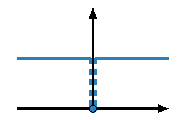
\includegraphics[width=\textwidth]{Figures/l0_regularizer.pdf}
         \caption{$\ell_0$}
     \end{subfigure}%
     \begin{subfigure}[b]{0.25\textwidth}
         \centering
         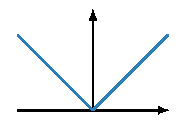
\includegraphics[width=\textwidth]{Figures/l1_regularizer.pdf}
         \caption{$\ell_1$}
     \end{subfigure}%
     \begin{subfigure}[b]{0.25\textwidth}
         \centering
         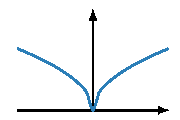
\includegraphics[width=\textwidth]{Figures/lh_regularizer.pdf}
         \caption{$\ell_p,\, p=1/2$}
     \end{subfigure}%
     \begin{subfigure}[b]{0.25\textwidth}
         \centering
         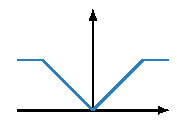
\includegraphics[width=\textwidth]{Figures/scad_regularizer.pdf}
         \caption{SCAD}
     \end{subfigure}
     \caption{Four commonly-used regularizers which promote sparsity}
     \label{fig:three graphs}
\end{figure}

\end{frame}

\begin{frame}{SR3-Relaxation for Mixed-Effect Models ($\ouralgo$)}
Original problem $\mathcal{FS-LME}$:
\eq{
	\min_{\beta \in \R^p,\, \gamma \in \R^{q}_+} \LL(\beta, \gamma) + R(\beta, \gamma)
}
Relaxed problem $\ouralgo$:
\eq{
	\label{eq:msr3_formulation_explicit}
	\min_{\beta, \tbeta \in \R^p,\, \gamma, \tgamma \in \R^{q}_+} \LL(\beta, \gamma) + \phi_\mu(\gamma) + \kappa_\eta(\beta - \tbeta, \gamma - \tgamma) + R(\tbeta, \tgamma)
}
where the \textit{relaxation} $\kappa_\eta$ decouples the likelihood and the regularizer 
\eq{
	\kappa_\eta(\beta - \tbeta, \gamma - \tgamma) := \frac{\eta}{2}\|\beta - \tbeta\|^2_2 + \frac{\eta}{2}\|\gamma - \tgamma\|_2^2, \quad \eta > \bar\eta
}
and the \textit{perspective mapping} $\phi_\mu$ replaces $\gamma \geq 0$ with a log-barrier 
\eq{
	\phi_\mu(\gamma) := \begin{cases}
		-\mu\sum_{i=1}^q \ln(\gamma_i/\mu), & \mu > 0 \\
		\delta_{\R_+^q}(\gamma), & \mu = 0 \\
		+\infty, & \mu < 0
	\end{cases}
} 
\end{frame}

\begin{frame}{Value Function Reformulation}
$\ouralgo$-relaxation replaces the original likelihood $\LL$ with a \textit{value function} $u_{\eta,\mu}$:
\eq{
	\label{eq:value_function_definition}
	v_{\eta,\mu}(\tbeta,\tgamma) & := \min_{(\beta, \gamma)} \LL_{\eta,\mu}((\beta, \gamma),(\tbeta, \tgamma)) \\  & := \min_{(\beta, \gamma)} \LL(\beta, \gamma) + \phi_\mu(\gamma) + \kappa_\eta(\beta - \tbeta, \gamma - \tgamma)
}
so $\ouralgo$-formulation~(\ref{eq:msr3_formulation_explicit}) becomes
\eq{
	\min_{\beta \in \R^p,\, \gamma \in \R^{q}_+} v_{\eta,\mu}(\tbeta, \tgamma) + R(\tbeta, \tgamma)
}
When $\eta$ is larger than the weak-convexity constant
\begin{itemize}
	\item $v_{\eta,\mu}$ is well-defined and continuously differentiable.
	\item As $\mu \rightarrow 0$ and $\eta \rightarrow \infty$, cluster points of solutions to $\ouralgo$ are first-order stationary points for $\mathcal{FS-LME}$ \\ 
	\item $v_{\eta, \mu}$ don't need to be evaluated precisely.
\end{itemize}

% \textbf{Key observation}: in practice, we don't need accurate solutions for~(\ref{eq:value_function_definition}): a few Newton iterations keep the solution close to the central path.
\end{frame}

%\begin{frame}{Value Function Reformulation}
%\begin{figure}
%	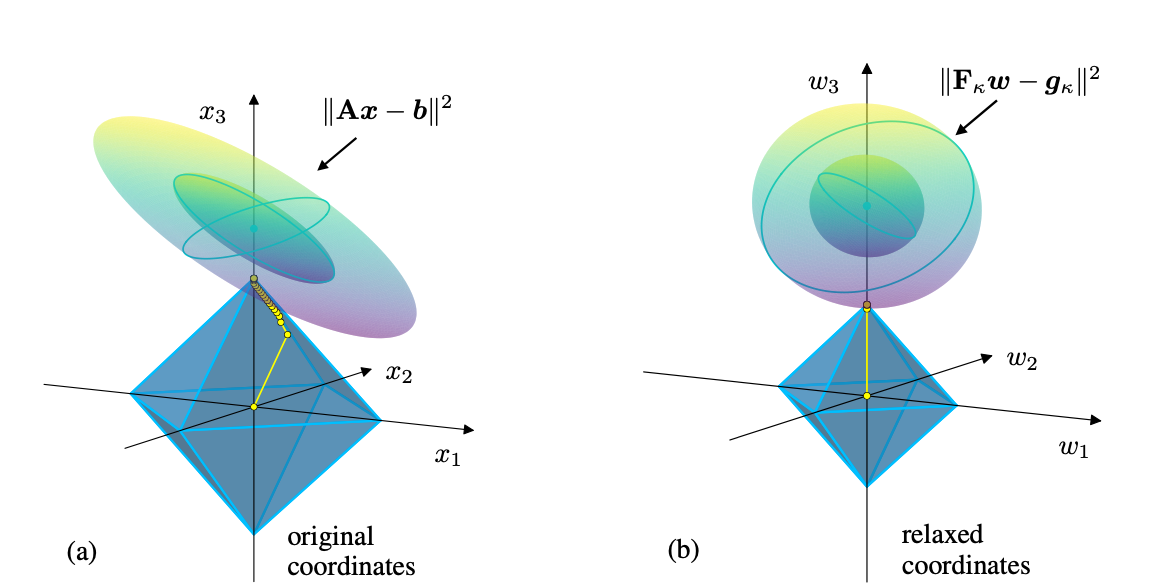
\includegraphics[width=\textwidth]{Figures/intuition_prev_paper}
%	\caption{\label{fig:intuition_prev} Picture from \cite{Zheng2018RelaxAndSplit}: for a linear problem, value function relaxation ``squashes'' level-sets simplifying the optimization landscape.}
%\end{figure}
%\end{frame}

\begin{frame}{Value Function Reformulation}
\begin{figure}
	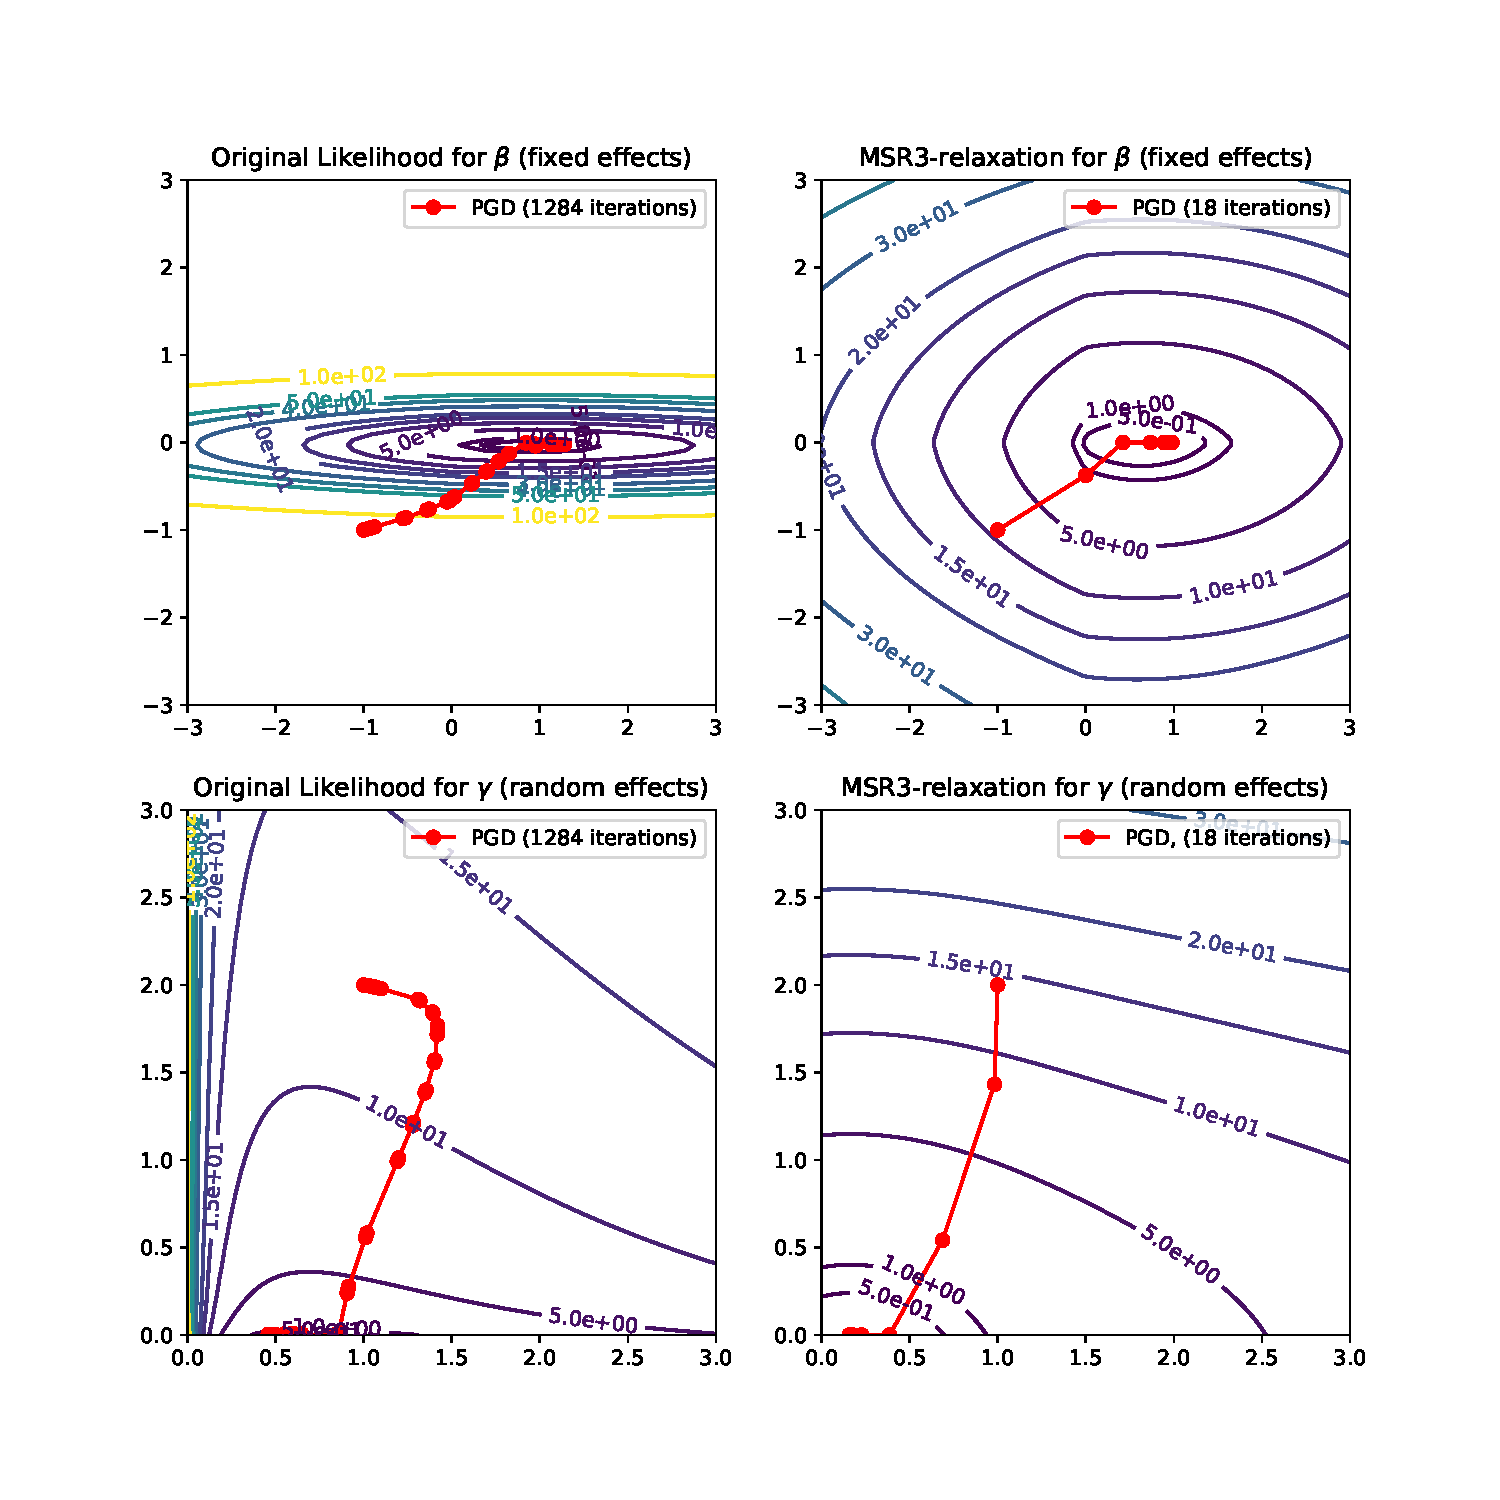
\includegraphics[width=0.7\textwidth]{Figures/intuition_current.pdf}
	\caption{\label{fig:intuition_sr3} Comparison of the level-sets for the original likelihood (left) and $\ouralgo$-likelihood (right), for fixed (top) and random (bottom) effects.}
\end{figure}
\end{frame}

\begin{frame}{Designing an Algorithm}
	$G_{\nu,\eta}$ encodes both gradient of a Lagrangian (lines 1-2) and the complementarity condition (line 3):
	\eq{
		G_{\nu,\eta}((\beta,\gamma,v),(\tbeta,\tgamma)) := \begin{bmatrix}
			\nabla_\beta \LL(\beta, \gamma) + \eta(\beta-\tbeta) \\
			\nabla_\gamma \LL(\beta, \gamma) + \eta(\gamma-\tgamma) - v\\
			v \bigodot \gamma - \mu\textbf{1}
		\end{bmatrix}
	}
	We apply Newton method to $G$ while geometrically decreasing $\mu$. \\
\textbf{Lemma:} For every $(\mu,\eta) \in \R_+\times\R_{++}$,
\eq{
	&(\hat\beta,\hat\gamma) = \argmin_{(\beta,\gamma)}\LL_{\eta,\mu}((\beta, \gamma),(\tbeta, \tgamma)) \\
	& \iff \\
	& \exists \hat{v} \in \R_{+}^q \text{ s.t. } G_{\nu,\eta}((\beta,\gamma,\hat{v}),(\tbeta,\tgamma)) = 0
}
If $\mu > 0$, then $\hat{v} = -\nabla\phi_\mu(\hat{\gamma})$, and if $\mu = 0$, then $\hat{v}$ is the unique KKT multiplier associated with the constraint $0 \leq \gamma$.
\end{frame}

\begin{frame}{$\ouralgo$-fast Algorithm}
\label{appendix:pseudocode}
\begin{algorithm}[H]
\SetAlgoLined
$\texttt{progress}\leftarrow \textbf{True}$; \quad \texttt{iter = 0}; \\
$\beta^+, \tbeta^+\leftarrow\beta_0$; 
\quad $\gamma^+, \tgamma^+\leftarrow\gamma_0$;  
\quad $v^+ \leftarrow 1 \in \R^q$; 
\quad  $\mu \leftarrow \frac{{v^+}^T\gamma^+}{10 q}$\\
 \While{\texttt{iter} $<$ \texttt{max\_iter}  \ and \ $\|G_\mu(\beta^+, \gamma^+, v^+)\|$ $>$ \texttt{tol}   \ and  \ \texttt{progress} \\}{
    $\beta \leftarrow \beta^+$; \quad $\gamma \leftarrow \gamma^+$; \quad $\tbeta \leftarrow \tbeta^+$; \quad $\tgamma \leftarrow \tgamma^+$ \\
%    $A \leftarrow \nbla G_\mu((\beta, \gamma, v), (\tbeta, \tgamma))$\\
  %  $b \leftarrow G_\mu((\beta, \gamma, v), (\tbeta, \tgamma))$\\
    $[dv, d\beta, d\gamma] \leftarrow  \nabla G_\mu((\beta, \gamma, v), (\tbeta, \tgamma))^{-1}  G_\mu((\beta, \gamma, v), (\tbeta, \tgamma))$
    $\alpha \leftarrow 0.99\times\min\left(1, -\frac{\gamma_i}{d\gamma_i}, \forall i :\ d\gamma_i < 0\right)$\\
    $\beta^+ \leftarrow \beta + \alpha d\beta$; \quad $\gamma^+ = \gamma + \alpha d\gamma$; \quad  $v^+ \leftarrow v + \alpha dv$\\
    \lIf{$\|\gamma^+\odot v^+ - q^{-1}{\gamma^+}^Tv^+ \mathbf{1}\| > 0.5q^{-1}{v^+}^T\gamma^+$}{continue}
    \Else{ 
        $\tbeta^+ = \prox_{\alpha R}(\beta^+)$;
        \    $\tgamma^+ = \prox_{\alpha R + \delta_{\R_+}}(\gamma^+)$; 
        \    $\mu = \frac{1}{10}\frac{{v^+}^T\gamma^+}{q}$
    }
%	\tcp*[h]{Keep iterating until convergence} \\
    \texttt{progress} = ($\|\beta^+ - \beta\| \geq \text{tol}$ or $\|\gamma^+ - \gamma\|  \geq \text{tol}$ or $\|\tbeta^+ - \tbeta\| \geq \text{tol}$ or $\|\tgamma^+ - \tgamma\| \geq \text{tol}$)\\
    \texttt{iter += 1}
 }
 \Return{$\tbeta^+$, $\tgamma^+$}
\end{algorithm}

\end{frame}

\section{Experiments}
\subsection{Application to Synthetic Problems}

\begin{frame}{Application to Synthetic Problems}
\begin{itemize}
	\item The number of fixed effects $p$ and random effects $q$ is 20.
	\item $\beta = \gamma = \frac{1}{2}[1,2,3,\dots,10, 0\dots,0]$
	\item 9 groups with sizes [10, 15, 4, 8, 3, 5, 18, 9, 6]
	\item $X_i \sim \NN(0, I)^p$, $Z_i = X_i$, $\varepsilon_i \sim \NN(0, 0.3^2I)$
	\item Each experiment is repeated 100 times.
	\item Grid-search for $\eta \in [10^{-4}, 10^{2}]$, golden search for $\lambda \in [0, 10^5]$
	\item Final model is chosen to maximize BIC
\end{itemize}
\begin{figure}
	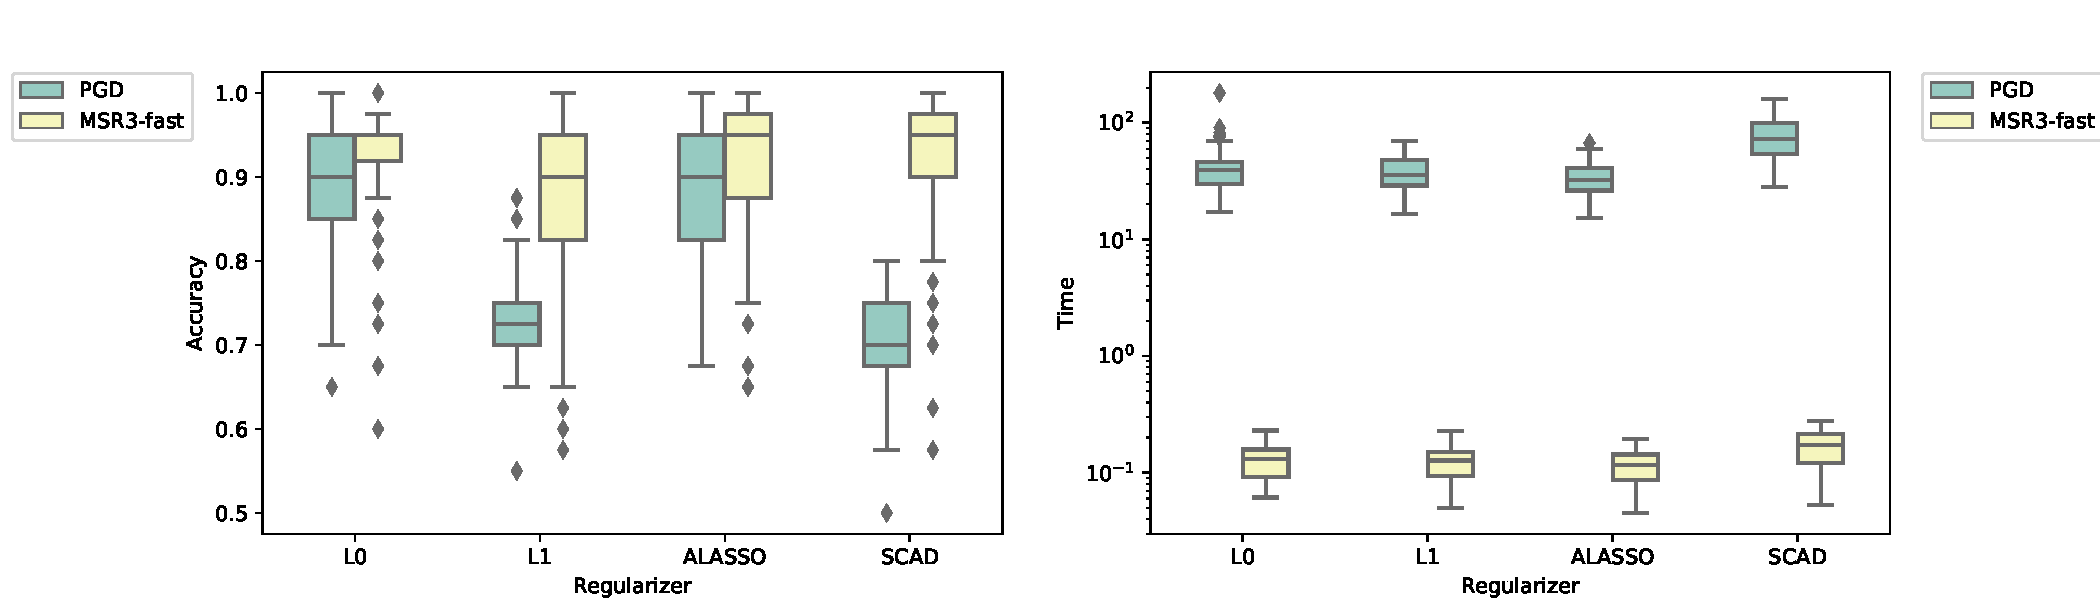
\includegraphics[width=\textwidth]{Figures/performance_without_msr3.pdf}
\end{figure}
\begin{itemize}
	\item[\textcolor{green}{+}] $\ouralgo$-relaxation improves feature selection performance of the original likelihood.
	\item[\textcolor{green}{+}] $\ouralgo$-fast optimization accelerates the compute time by $\sim 10^2$.
   	\item[\textcolor{red}{--}] Initialization of $\eta$ is problem-specific
\end{itemize}
\end{frame}

\begin{frame}{Comparison to Other Libraries}
\begin{table}
	\begin{tabular}{lrrrr}
\toprule
Algorithm &        MSR3-Fast ($\ell_1$)&         \texttt{glmmLasso}\footnote{\href{https://rdrr.io/cran/glmmLasso/man/glmmLasso.html}{https://rdrr.io/cran/glmmLasso/man/glmmLasso.html}} \cite{groll2014variable}  &            \texttt{lmmLasso}\footnote{\href{https://rdrr.io/cran/lmmlasso/}{https://rdrr.io/cran/lmmlasso/}}\cite{schelldorfer2011estimation} & PGD ($\ell_1$) \\
\midrule
Accuracy, \% &     {\bf 88} &        48 &          66 & 73  \\
FE Accuracy, \% &      {\bf 86} &        52  &          47 & 56\\
RE Accuracy, \% &     {\bf 91} &        45  &         84 & {\bf 91} \\
Time, sec        & {\bf 0.19} &  1.37  &  11.51 & 38.39 \\
Iterations, num  &      34 &        50 &             - & 7693 \\
\bottomrule
\end{tabular}
\end{table}
\end{frame}

\begin{frame}{Choice of $\eta$}
	\begin{figure}
		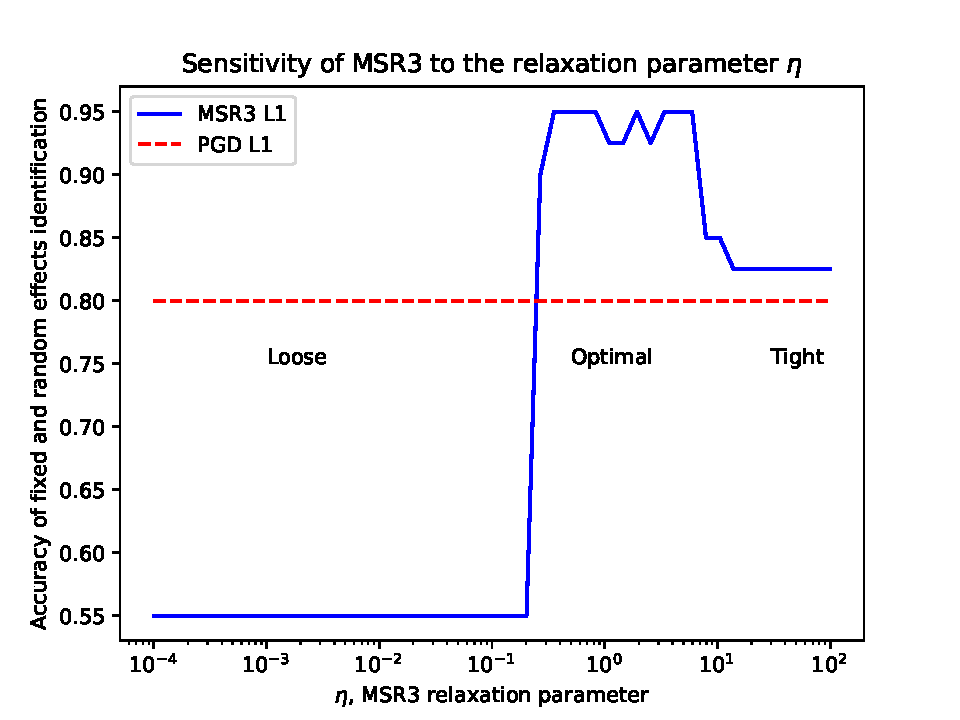
\includegraphics[width=\textwidth]{Figures/eta_L1.pdf}
	\end{figure}
\end{frame}

\begin{frame}{$\ell_0$-based Covariate Selection for Bullying Study from GBD}
	\begin{figure}
		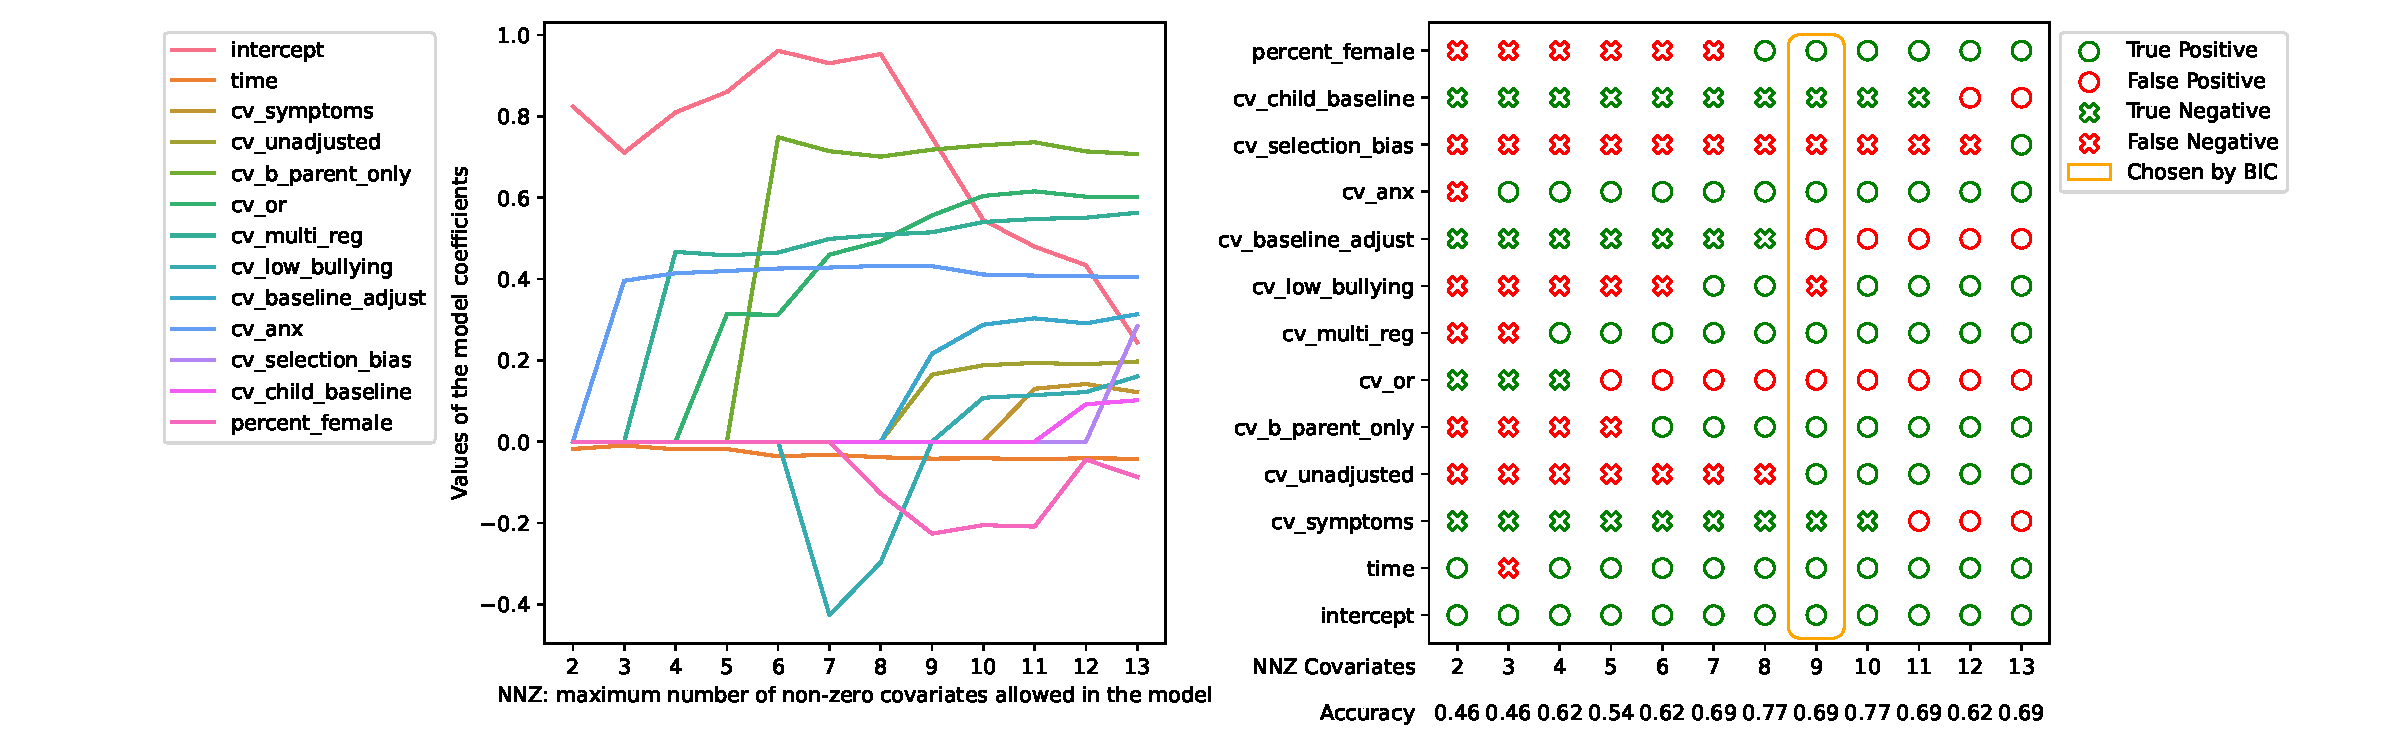
\includegraphics[width=\textwidth]{Figures/bullying_data_assessment_selection.pdf}
		\caption{Fixed and random covariate selection for Bullying dataset from~\cite{GBD}. The model selected 9 covariates, 7 of which were historically significant, and did not select 4 covariates, 1 of which was historically significant.}
	\end{figure}
\end{frame}

\begin{frame}{Software}
	The code is available on GitHub: \href{github.com/aksholokhov/pysr3}{https://github.com/aksholokhov/pysr3}
	\begin{itemize}
		\item All estimators are fully compatible to \texttt{sklearn} library.
		\item Implements SR3 for linear, generalized-linear, and linear mixed-effect models.
		\item Has tutorials, tests, and documentation.
	\end{itemize}
\end{frame}
